\chapter{FINDINGS}
\begin{figure}[ht!]
    \centering
    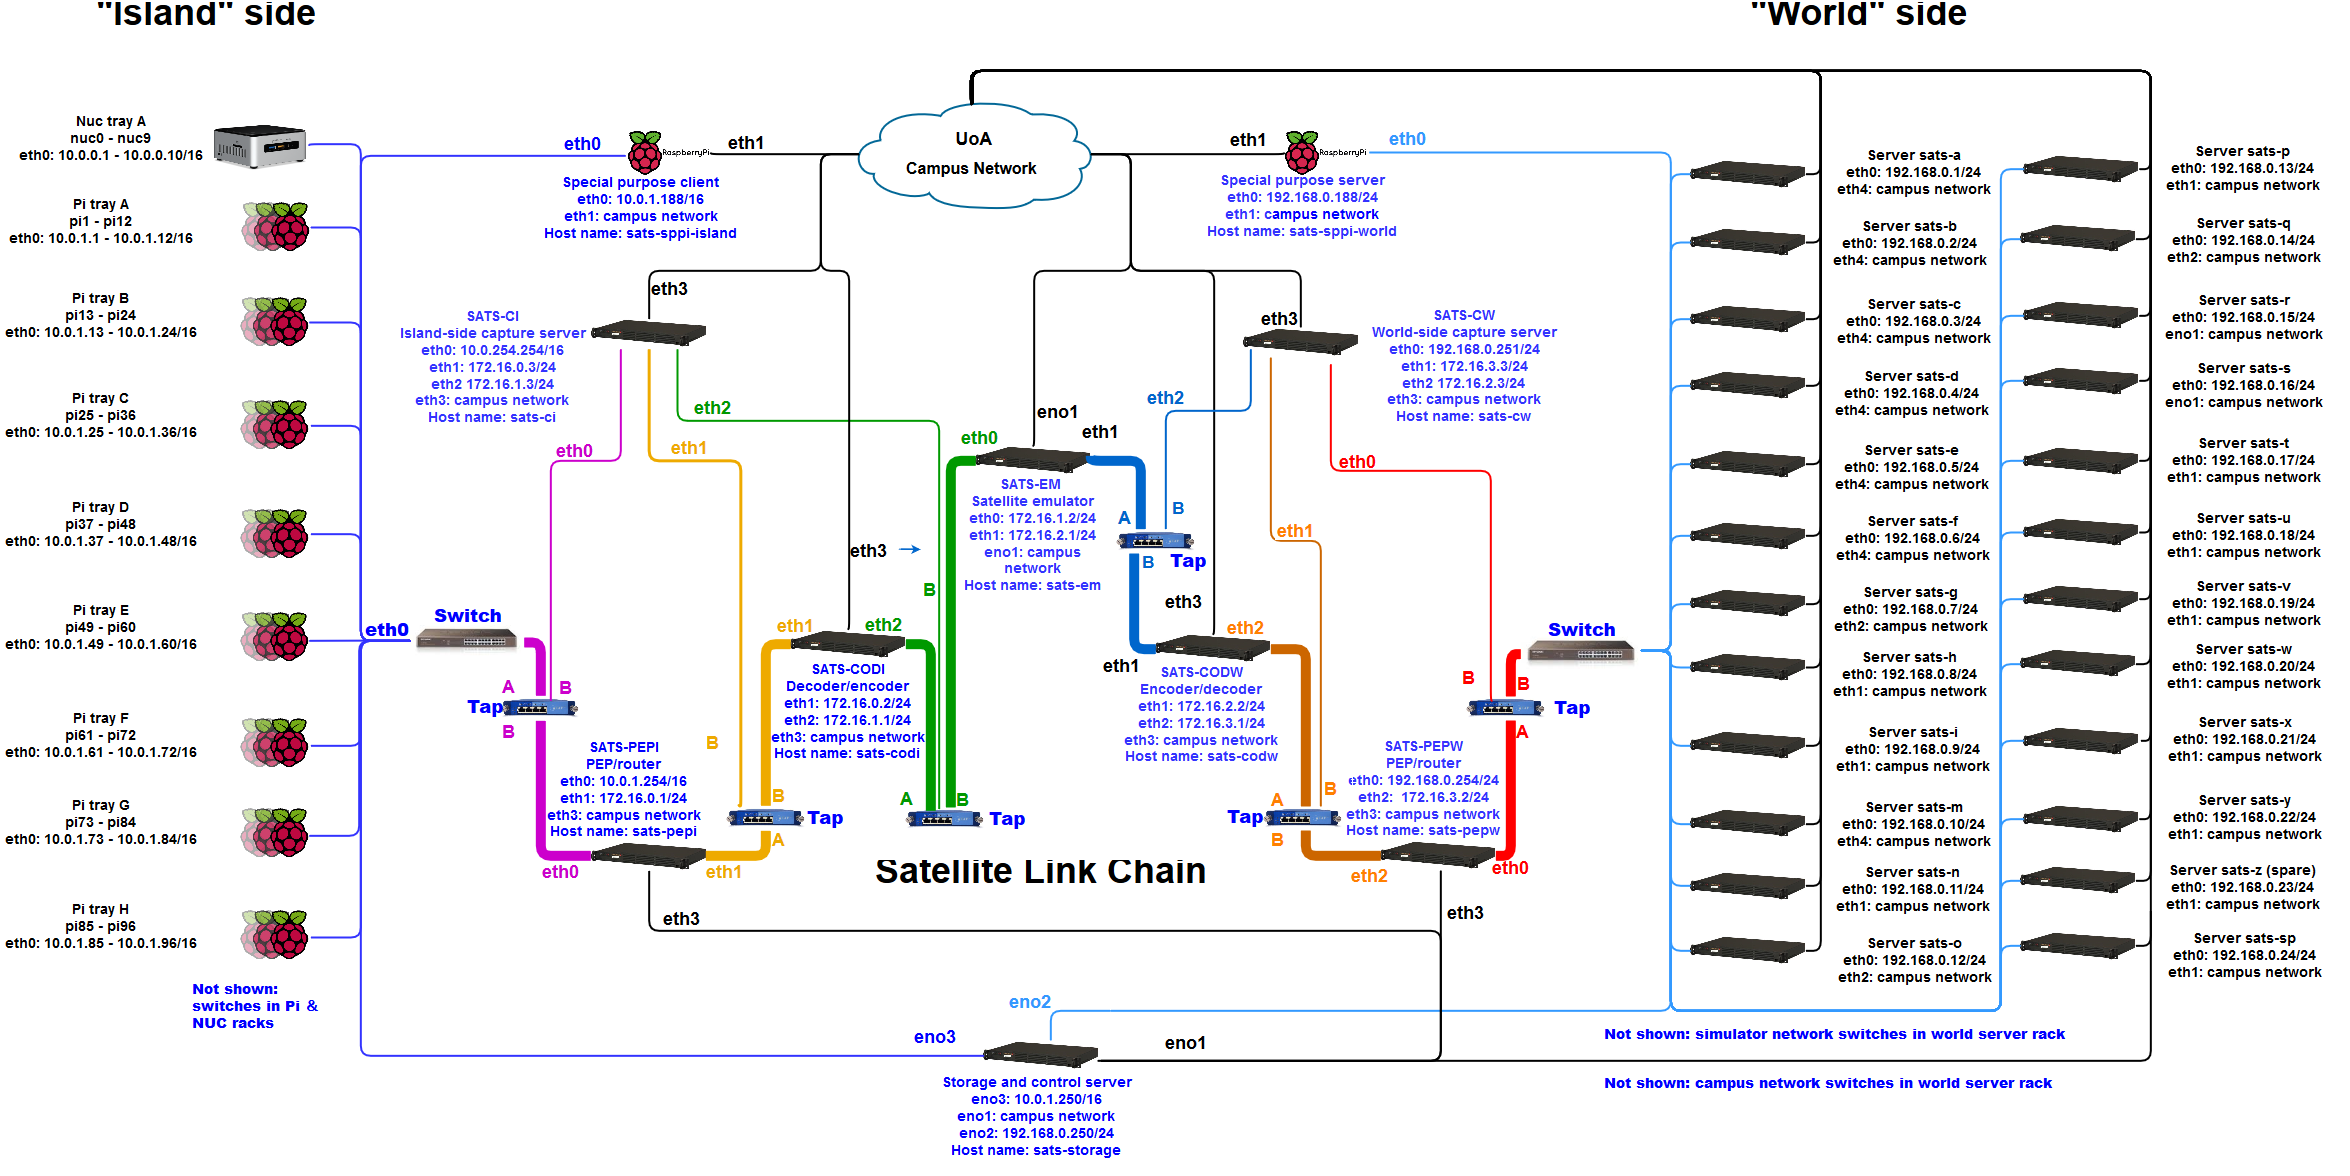
\includegraphics[width=1.3\textwidth, angle =270]{Simulator.png}
    \caption{Pacific Island Satellite Simulator Topology. }
    \label{fig: Satellite Simulator} 
\end{figure}

This section will be looking at the findings when we tested the PEP on the University of Auckland's (UOA) Pacific Island Satellite Simulator. These findings are compared to the PEPsal results conducted previously obtained on the same testbed by a PhD student- Quan and Professor Speidel. The road to get to this testing stage, however, was paved with many challenges. Section ~5.1 will look at the Pacific Island Satellite Simulator testbed before we look at the testbed experiment results in Section 5.2 and discuss the positives and negatives. \todo{make sure the section headings align} \\

\section{Pacific Island satellite testbed}
Figure 5.1 shows the general topology of the simulator.The simulator consists, in principle, of four networks. These four networks are represented on Fig 5.1 by the four different line colours. Each machine connected via the same coloured line is part of the same network and can see all other machines on the network directly without the aid of a router ~\cite{21}. \\

\subsection{Simulator topology and the technology within the simulator}
The testbed is divided into two halves. On the left side, connected by the thin light blue lines/network, we have the island side which represents the terrestrial hosts on the Pacific island. This left-hand side of the testbed consists of 96 Raspberry Pis and a tray of mini NUC PCs with SSD and a small amount of memory. The NUCS and Raspberry Pis run on the light blue private network which can be seen to the left of the Pis in Fig 5.1. These machines are simulating the clients sitting on the island side that will be connecting and receiving data from the servers on the world side (right-hand side of the topology). Their job is not very computing intensive as they only need to record the amount of data received and the time it arrived, hence the use of raspberry pis and NUCs ~\cite{21}. \\

On the right side, connected by the thin dark blue lines/network, are the machines representing terrestrial hosts from the world side on the other side of the satellite link. This side consists of 24 devices acting as the servers of the world in the simulated "world" network. 22 of these machines are actively simulating servers of the world, 1 of them of them is a special purpose server, and the last one is a spare machine to be used in case one fails. Standard switches connect these machines. They will receive socket connection requests from the clients on the island side and reply with data ~\cite{21}. \\

Right in the middle near the centre of the page, we have the satellite emulator SATS-EM which represents the geostationary satellite providing Internet access from the world side to the island side. This machine (SATS-EM) simulates the bandwidth constraints and latencies of the narrowband satellite link. For example, on a 16Mbps geostationary satellite link, it ensures that the data rate going through is only 16Mbps as per the real link and simulates the satellites link latencies and queue input capacities to the satellite. The thick multicoloured lines running through the satellite (SATS-EM) from the left "island" side through to the right "world" side, represents the bottleneck satellite link chain. This chain contains four further machines that by default are all configured to act as forwarding routers unless they are given a specific task ~\cite{20}~\cite{21}.\\

SATS-PEPI is the \emph{island-facing router/PEP} machine connected by the thin light blue lines to the left-hand side, and SATS-PEPW is the \emph{world side facing router/PEP} connected by the thin dark blue lines to the right-hand side. While the simulator allows for PEPs to be set up in a distributed architecture on both sides of the degraded satellite link, only the \emph{world side facing router/PEP} is being used as a performance enhancing proxy ~\cite{4}~\cite{5}~\cite{21}. The SATS-PEPI can be treated as a standard vanilla router for forwarding traffic in our case (integrated architecture). The reason for this is because in our experiments, practically all of the traffic payload data will be coming from the world-side to the islands hosts so there is no benefit from having a PEP configured on the island side ~\cite{21}. This has been configured this way just for ease of experimentation measurements but in a real world scenario, we would use a distributed architecture. The two switches between the PEPs and their island sides/world sides are simulating ground station equipment.\\ 

Between the PEPs and the SATS-EM (satellite emulator), we have two machines SATS-CODI and SATS-CODW which are decoders and encoders for network coding. Our experiments do not use network coding, so they act as plain vanilla routers in this case. We also have six copper taps along various points of the satellite link. They are used to capture and copy traffic and feed data directly to server SATS-CI  (island-side capture server) and SATS-CW (world-side capture server) for processing, shown in Figure 5.1 via the thin multicoloured lines ~\cite{20}~\cite{21}. \\

Right at the bottom of Figure 5.1, towards the centre of the diagram, is the storage and control server which controls the experiment. It is connected to the campus network via the thin black lines in the picture. The campus network sits outside our simulated satellite network so we can make configuration/software changes and check the experiments externally. This external access allows for changes to be made to the operation and for interaction with the world side servers without causing interference to the test ~\cite{21}. \\

Finally, we have the two Raspberry Pis located at the top of Figure 5.1 that act as two special purpose client and server Pis. These Pis send ICMP pings at the start of the experiment and then again at the end. These pings are visible in all traces taken along the satellite chain. When the PEP processes the data, these pings identify the start and end of an experiments captured data for better data analysis accuracy ~\cite{21}. 

\subsection{Basic rundown of the experiment}
On the island side, we have a client program that is run on the NUCs and the Raspberry Pis. This program involves the use of \emph{channels} which are defined as TCP socket connections that are repeatedly made between a client on the island side to a randomly selected server on the world side in a sequential order. We configure each client program with a certain number of these channels. A count is done on all the channels configured for all the NUCs and Pis and this allows us to control the load on the satellite link. Once the connection has been made, the server sends the island-side client a certain amount of data (as determined by the sender from a known flow size distribution collected from the Cook Islands) and then the socket connection is ended. The client channel then repeats the process and opens a new TCP socket connection to another randomly selected server. This process is repeated until the experiment times out ~\cite{21}. \\

The special purpose server (SATS-SP) located on the world side has a special purpose in our experiment. Since our clients randomly select the servers and the amount of bytes the servers send back to the clients is also randomly selected, it is possible only to get small or medium size transfers. The SATS-SP guarantees we get a large size transfer across our simulated network link. When the experiment starts, the SATS=SP connects to an iperf3 server on one of the NUCs and then transfers a significant amount of data ~\cite{21}. In our experiment, this nominal transfer is 40MB. \\

The SATS-SP also pings continuously at the start of the experiment, at rate of ten times per second. The ping packets are ideal because they are accepted into the byte queue at the input of the satellite link, even when the link is congested and the queue is overflowing with larger packets. Their tiny size means they can squeeze in at the end of the queue where larger data packets cannot ~\cite{21}.\\

The following is a basic rundown of the experiment procedure:

\begin{enumerate}

\item Test the system. Test the connectivity to make sure all servers can be pinged. We control the experiment via the external campus network so as to not contaminate the experiment traffic (storage and control server). 
\item Compute how we are going to distribute the requested number of channels among the Pis and NUCs. Automatically generates a script which starts up the Pis and NUCs and shuts them down.
\item Start capturing at the tap nearest the island-side and continue along the rest of the taps. The idea is that any data/packets captured at one tap and not showing in the next one can be assumed lost somewhere along the satellite chain. Start capturing at the tap nearest the world side. 
\item Start the world servers then start the clients (island-side). Let them both ramp up for ten seconds.
\item Start the iperf3 server on one of the NUCs. Note that in iperf3, the client sends data to the server rather than downloading it.
\item Send special client ping after ten seconds to signal the start of the experiment.
\item Start pinging and iperf3 transfer. Each experiment will run for approximately 600 seconds. (120 experiments will run in one batch).
\item  The special server world-side sends an \emph{end} pings after approximately 600 seconds of experiment time.
\item Shut down the iperf3 client, island clients and world servers.
\item Retrieve trace files collected by the taps from both capture servers and the iperf and ping logs from the world side special purpose server.
\item Collect data analysis from storage server and render onto graph.\\
\end{enumerate}

In the next section, we look at three different graphs yielded from three different batches of these experiments. Each batch contains 120 individual experiments which take roughly 15 to 30 minutes each to perform. We ran the experiments with load levels of between 10 to 120 channels and for each load level we ran 10 experiments ~\cite{21}. \\

We will perform the same batch of experiments on three different variations of our PEP. The only difference will be in the PEP input queue capacity and its retransmission times as can be seen in the next section.\\

For each of these three experiments, there was already an existing dataset of equivalent baseline and PEPsal experiments that we are using for comparison here ~\cite{4}~\cite{21}. 

\section{Running the PEP on the Satellite Simulator}
In the three graphs presented in this section, we have three data series in each graph as represented by three colours. Black represents baseline (no PEP), blue represents PEPsal, and the red the results of our PEP. The x-axis represents the client load we are putting on the link, measured in channels. The left y-axis marked with crosses represents total goodput. \\


\begin{figure}[ht!]
    \centering
    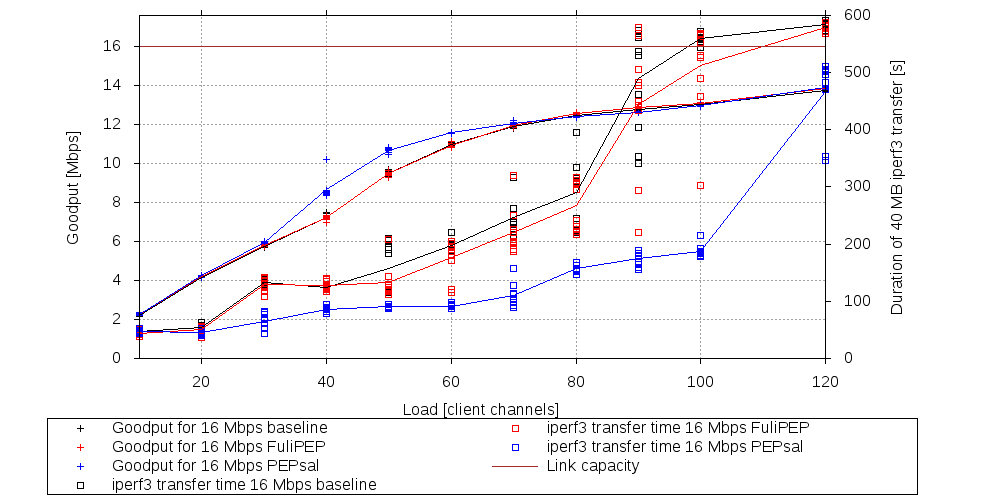
\includegraphics[width=1.3\textwidth, angle =270]{120K.png}
    \caption{Satellite link input queue capacity 120 kB, maximum RTT estimated as 1.3 * measured RTT of last ACK.}
    \label{fig: 120K queues} 
\end{figure}

Normally, total goodput is defined as the rate by which \emph{useful data} traverses the link, but in our experiment, our simulator measures total goodput as the rate of TCP payload data arriving at the other end of the link. Here, we want the total goodput to be as high as possible of course. \\

In the case of our PEP, this may include premature retransmissions, which normally would not be accounted for under goodput. However, due to the way the simulator operates and the fact that it is somewhat difficult to get the goodput from a large number of flows, we are constrained to having this as a possible adverse side effect. \\

Each individually coloured box represents the \emph{total iperf3 transfer} time for one experiment (y-axis). A good PEP result is when this transfer time is as low as possible indicating that data is capable of being transported faster across the link. The different coloured crosses represent the \emph{total goodput} for each experiment.\\

\begin{figure}[ht!]
    \centering
    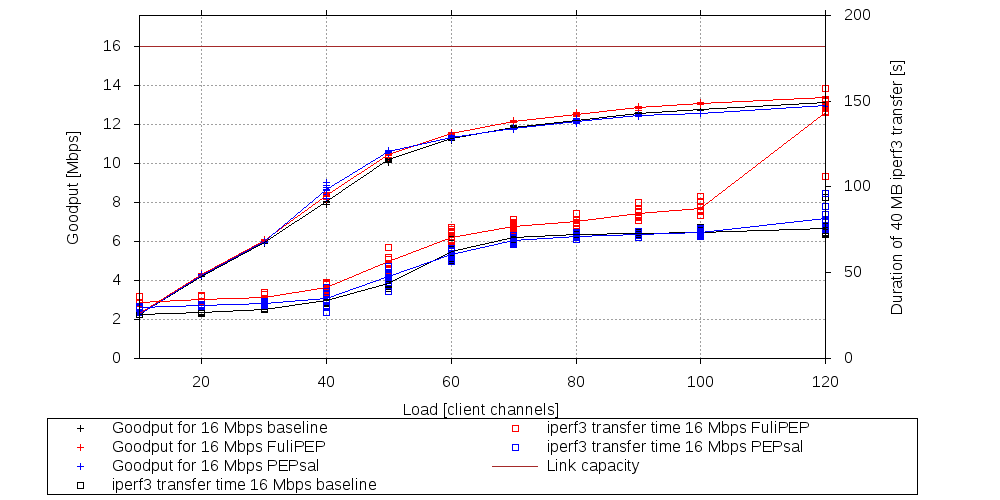
\includegraphics[width=1.3\textwidth, angle =270]{2000k.png}
    \caption{Satellite link input queue capacity 2000 kb, maximum RTT estimated as 1.3 * measured RTT of last ACK.}
    \label{fig: 2000k} 
\end{figure}

Figure 5.2 shows the results obtained from 120 experiments over varying loads when testing our PEP with a satellite link input queue capacity of 120k and a maximum RTT estimated as 1.3 x measured RTT from the last ACK. Recall that this dynamic recalculation of RTT affects the retransmission time for packets waiting in the cache. Hence the lower the multiple of RTT, the earlier our PEP will send retransmissions across the link. As mentioned above, however, this could affect the goodput in our experiment as it may result in more retransmissions.\\

We observe that the total goodput in our PEP is nearly identical to baseline (no PEP) and comparable to that of PEPsal except in the mid-load range between 30 and 70 client channels, where PEPsal is up to about 20 percent ahead.\\

For the individual iperf3 transfer, it is evident that our PEP performs better than baseline from about 50 client channels onwards, but it falls well below matching PEPsal's results just yet. Hopefully, our PEP will outperform PEPsal in the future once we can adjust the code to keep track of what is on the link and adjust the receiver's advertised window (rwnd) accordingly (see future work section in the next chapter).\\

\begin{figure}[ht!]
    \centering
    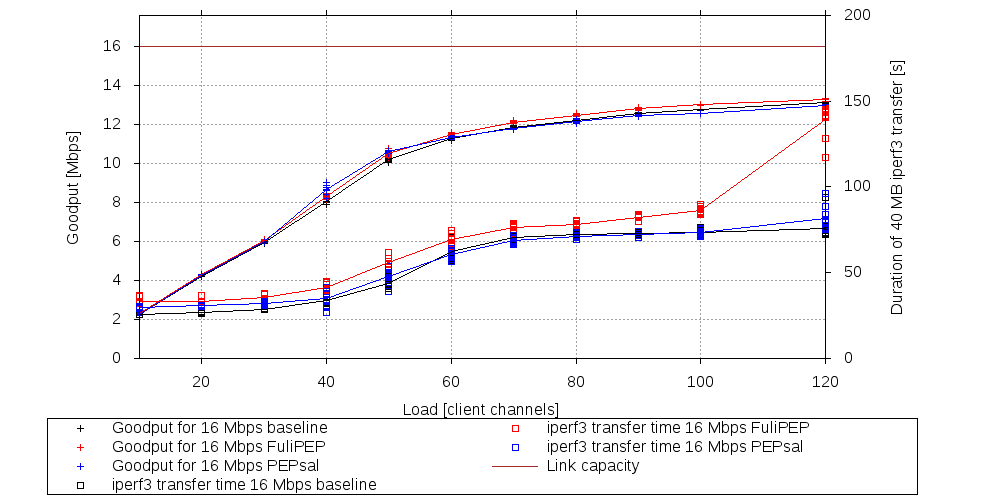
\includegraphics[width=1.3\textwidth, angle =270]{2000k-2.png}
    \caption{Satellite link input queue capacity 2000 kB, maximum RTT estimated as 2 * measured RTT of last ACK.}
    \label{fig: 2000k + 2*RTT} 
\end{figure}

Figure 5.3 shows the results obtained from 120 experiments over varying loads when testing our PEP with a satellite link input queue capacity of 2000kb (conventionally recommended queue capacity) and a maximum RTT estimated as 1.3 x measured RTT after last ACK. Total goodput, in this case, starts to slightly exceed PEPsal at around the 60 load channel mark and also performs above baseline across the board. While the PEP has an extra few percent of total goodput, some of this could theoretically be due to retransmission duplicates being counted as goodput (we only count TCP payload bytes), but if this is not the case, then the results are positive. For the individual iperf3 transfer, however, both the PEP and PEPsal have worse (more extended) transfer times than baseline. This will hopefully improve with future modifications to the PEP (see future work section in the next chapter). \\

Figure 5.4 shows the results obtained from 120 experiments over varying loads when testing our PEP with a satellite link input queue capacity of 2000kb (conventionally recommended queue capacity) and a maximum RTT estimated as 2 x measured RTT after the last ACK. The results are almost exactly identical to the previous experiment in Figure 5.2. From this result, we can tentatively conclude that the goodput is being measured accurately because the changes made to estimated RTT and the subsequent frequency of retransmissions have seemingly no effect on the results. If the retransmissions were a significant part of the goodput, we would expect to see a markedly different result when we change from 1.3 x RTT to 2 x RTT. The link input queue capacity seems to be the only variable in these three graphs that makes a discernible difference to the results. 